\documentclass{IAYCPro}

\projectyear{2024}
\projectauthor{\large Konstantinos Kilmetis (s3745597) \& Diederick Vroom (s2277387)}
\projectname{Computational Physics: Molecular Dynamics}
\projectgroup{COP 2024}

\projectstartpage{1}
\usepackage[latin1]{inputenc}
\usepackage[english]{babel}
\usepackage{gensymb}
\usepackage{graphicx}
\usepackage{verbatim}
\usepackage{wasysym}
\usepackage{marvosym}
\usepackage{lmodern}
\usepackage{hyperref}
\usepackage{siunitx} %\si{km.s^{-1}} unit
\usepackage{mathtools} %\Aboxed{} for box
\usepackage{chngcntr} %For using split environment --> give equations in align environment 1 reference label
\counterwithout{equation}{section} %Count equation labels independently of section numbers. I.e. no longer equation (3.14) (equation 14 in section 3), instead it is a whole number, e.g. equation (42) (42nd equation in the entire document).
\usepackage{multirow}
\usepackage{subcaption}

\newcommand{\dd}{\mathrm{d}} %For easily writing differentials
\newcommand{\ssi}[1]{\;\si{#1}} %automatically put a space before using units with \si{}

% Fonts
\usepackage{fontspec}
\newfontfamily\droid[
  Path = fonts/ ,
  UprightFont = *-Regular,
  BoldFont = *-Bold,
  ItalicFont = *-Italic,
  BoldItalicFont = *-BoldItalic,
  Extension = .ttf
  ]{DroidSerif}
\setmainfont{DroidSerif}
\usepackage{listings}

%This is a skeleton file for typesetting source code ---using the LaTeX listings package--- for the Computational Physics course 2019-2020.
%Tested and compiles using pdflatex, lualatex and xelatex.

%The following settings are copied from Wikibooks (https://en.wikibooks.org/wiki/LaTeX/Source_Code_Listings) and slightly adjusted:
\lstset{ 
  backgroundcolor=\color{white},   % choose the background color; you must add \usepackage{color} or \usepackage{xcolor}; should come as last argument
  basicstyle=\footnotesize,        % the size of the fonts that are used for the code
  breakatwhitespace=true,          % sets if automatic breaks should only happen at whitespace
  breaklines=true,                 % sets automatic line breaking
  linewidth=\linewidth,            % sets the linewidth of the code frame to the linewidth of the document
  commentstyle=\color{gray}\itshape, % make comments gray and italic 
  captionpos=b,                    % sets the caption-position to bottom
  deletekeywords={...},            % if you want to delete keywords from the given language
  escapeinside={\%*}{*)},          % if you want to add LaTeX within your code
  extendedchars=true,              % lets you use non-ASCII characters; for 8-bits encodings only, does not work with UTF-8
  firstnumber=1,                   % start line enumeration with line 1000
  frame=single,	                   % adds a frame around the code
  keepspaces=true,                 % keeps spaces in text, useful for keeping indentation of code (possibly needs columns=flexible)
  language=Python,                 % the language of the code
  morekeywords={as, self, Dict, Tuple, List, Any, Union, None, ...},            % if you want to add more keywords to the set
  numbers=left,                    % where to put the line-numbers; possible values are (none, left, right)
  numberstyle=\tiny,               % line numbers are smaller
  numbersep=5pt,                   % how far the line-numbers are from the code
  rulecolor=\color{black},         % if not set, the frame-color may be changed on line-breaks within not-black text (e.g. comments (green here))
  showspaces=false,                % show spaces everywhere adding particular underscores; it overrides 'showstringspaces'
  showstringspaces=false,          % underline spaces within strings only
  stringstyle=\color{gray},        % strings are also gray
  showtabs=false,                  % show tabs within strings adding particular underscores
  stepnumber=1,                    % the step between two line-numbers. If it's 1, each line will be numbered
  tabsize=2,	                   % sets default tabsize to 2 spaces
  title=\lstname                   % show the filename of files included with \lstinputlisting; also try caption instead of title
}

\begin{document}
\begin{center}
    \textbf{Abstract}
\end{center}
\vspace{-1em}
Through the usage of molecular dynamics simulations, emergent properties of Argon atoms in different states of matter is calculated. Assuming that the Argon atoms interact through a Lennard -- Jones potential, and periodic boundary conditions, we are able to calculate the pressure and the pair correlation function (PCF). The parameter space of the phase diagram is explored and the triple point of Argon is calculated to be at (T,P) = (90 K , 10$^{\text{-4}}$ GPa) 

\section{Introduction}
\label{sct: Introduction}
The dynamics of individual atoms of any species are impossible to calculate analytically. Their emergent behaviour becomes chaotic, in the same fashion that the three-body problem becomes. Indeed, they are more complex than the three-body problem since gravity is a purely attractive force, while the electromagnetic interactions which govern molecular dynamics attract and repel. \\ \\
Despite that, there is much to be learned by studying such systems. A lot of questions are open, from the behaviour of molecules in extreme conditions to the nature of protein structure. In this work we will be focusing in a much more constrained case; the phases of Argon. \\ \\
Argon's inert\footnote{one might say, noble} nature, makes it ideal for a proof of concept calculation. We assumed that each atom interacts with one solely through the Lennard -- Jones potential, expressed in Eqn. \ref{eq:LJ},
\begin{equation}
    \label{eq:LJ}
    V_\text{LJ}(r) = 4\varepsilon \left[ \left( \frac{\sigma}{r} \right)^{12} - \left( \frac{\sigma}{r} \right)^6 \right].
\end{equation} 
It is described by two terms. The attractive \textit{van der Waals} term, scaling with $r^{-6}$, and the repulsive \textit{Pauli} term, scaling with $r^{-12}$. Intuitively, these two combine to form a mildly attractive central force, which becomes fiercely repulsive in very short scales. \\ \\
Said scales are described by the $\sigma$ and $\varepsilon$ factor. Respectively they correspond to the size of each particle and the minimum energy. They identify the species of each particle, in our case they all take the Argon values of $\sigma = 3.405$ \r{A} and $\varepsilon = 119.8$ $k_\text{B}$ K. 

\raggedbottom
\newpage

\section{Methods}
\label{sct: Methods}
The Lennard -- Jones assumption implicitly ignores any quantum dynamical effects. By making it we assume that any such effects have such a minute influence on the system, so much so that they may be safely ignored. Then we are left with Newtonian Dynamics. The equations which we need to solve are only the classical motion equation for each particle $i$, shown below: 
\begin{equation}
    \label{eq:newton}
    m_\text{Ar} \frac{d^2 \vec{x}_i}{dt^2} = -\sum_j \nabla V_\text{LJ}(\vec{x}_i - \vec{x}_j),
\end{equation}
the fact that the Lennard -- Jones potential is central works to our advantage here. The equation has only to be integrated in the radial directions, since the potential does not predict any force in non-radial directions. Then, can then be simplified as follows,
\begin{equation}
    \label{eq:onedim}
    \vec{F}(\vec{x}_i) = -\sum_j \nabla V_\text{LJ} \left( \bigg| ||\vec{x}_i|| - ||\vec{x}_j|| \bigg| \right).
\end{equation}
Admittedly this is denser notation, put it is simpler to compute.
% Kon: make sure to mention verlet, MIC, FCC, velocity rescaling
\subsection{Integration Scheme}
There is an abundance of ways to integrate Eqn. \ref{eq:onedim} but not all of them have desirable properties. What concerns us the most is the conservation of energy. By Noether's theorem we know that since the system is symmetric with regard to time -there is no explicit time dependence our potential- energy should be conserved. To achieve this we employ the \textit{velocity Verlet} integrator. \\ \\
Any numerical solution will diverge from the true solution due to truncation errors. This is a natural consequence of the limited amount of accuracy any computation on limited memory has. Verlet's algorithms also known as leapfrog take advantage of the time-symmetric nature of the problem to cancel these errors out. \\ \\
This is achieved by taking an initial half step before starting the full calculation. By doing so and subtracting, we both get rid of $\mathcal{O}(h^2)$ terms and introduce time-symmetry. Our calculations still come with a significant $\mathcal{O}(h^3)$ error, but every step it oscillates between underestimating and overestimating the true energy. It doesn't diverge. During the half step, we could either check the new position or velocity during the half step, we chose velocity. Thus, this leaves us with the following equations to evolve:
\begin{align}
    % \Vec{v}\left(t + h \right) &= \vec{v}\left(t\right)\frac{3h}{2m_\text{Ar}} \left( \vec{F}(\vec{x}) + \vec{F}(\vec{x}) \right) + \mathcal{O}(h^3)
    \vec{v}\left(t+g\right) &= \vec{v}(t) + \frac{h}{2m_\mathrm{Ar}}\left[\vec{F}\left(x(t+h)\right) + \vec{F}\left(x(t)\right) \right] + \mathcal{O}(h^3)
    \label{eqn: Verlet Vel}
    \\
    \Vec{x}\left(t + h\right) &= \vec{x}\left(t \right) +  h\vec{v}\left(t \right) + \frac{h^2}{2m_\text{Ar}} \vec{F}(\vec{x}(t)) + \mathcal{O}(h^3)
    \label{eqn: Verlet Pos}
\end{align}

\raggedbottom
\newpage

\subsection{Boundary Conditions}
To approximate even a tiny quantity of Argon, we would need to simulate a number of atoms close to Avogadro's number. In the interest of computational expediency we only simulate 108 Argon atoms. In order to both circumvent the need to resolve collisions from firm boundaries and approximate an infinite quantity of Argon, we employ a periodic boundary condition. We seek to copy and paste our cube of 108 particles to all directions, so our original 108 particles are embedded in a wider sea of Argon. Again this conflicts with our desire for computational expediency. \\ \\
Enter, minimal image convention. It stipulates that, when calculating the distance from particle A to particle B, only use the copy of particle B which lies closest to particle A. Since we know that the maximum distance between particles in one dimension is half the box size; if the copy within the box is less than half a box length away, then this is the closest one. If the copy within the box lies at a distance $d$ more than half a box length away, the closest copy would be $L/2 - d$. We can implement it through the following one liner, which we repeat for every dimension.
\\
\lstinputlisting{MIC.py} 
That way we can simulate 108 particles, while pretending that they are surrounded by a sea of particles. A corollary of the minimum image convention is the \textit{pacman}-esque behaviour of our boundary. When a particle leaves from the left side, it reappears on the right one.

\subsection{Initial Conditions}

Our goal for this project is to simulate a collection of Argon atoms in the three phases of matter: Gas, liquid, and solid. Picking the right initial densities and temperatures should be all that is required to observe Argon in these phases. In the real world this might suffice, however, in simulation world this is an enormous bottleneck. Wanting to observe the phases of Argon in this manner requires letting our system settle until it naturally forms the structures corresponding to the different phases. A process which takes seconds in the real world, but can take billions of iterations in simulation world. Hence, we have to be clever about our initial conditions. Our initial conditions consist of two parts: the initial positions of the Argon atoms and their velocities. For both of these conditions, we let the real world nudge us in the right direction. 

\raggedbottom
\newpage

\subsubsection{Position}

At first thought, the initial positions of the Argon atoms should be totally random and uniformly distributed. But we know from lab experiments and theory that this is not the case. The atoms interact and therefore have a preferred configuration, which minimizes the total energy of the system. This configuration differs for each state of matter, but does follow a structure. For gas phase Argon, we would expect each atom to have high kinetic energy and thus our collection of atoms to be relatively homogeneously distributed in the container box. For solid phase Argon, the atoms form a crystal structure going by a Face-Centred Cubic (FCC) design, see Fig. \ref{fig: FCC}. 

\begin{figure}[H]
    \centering
    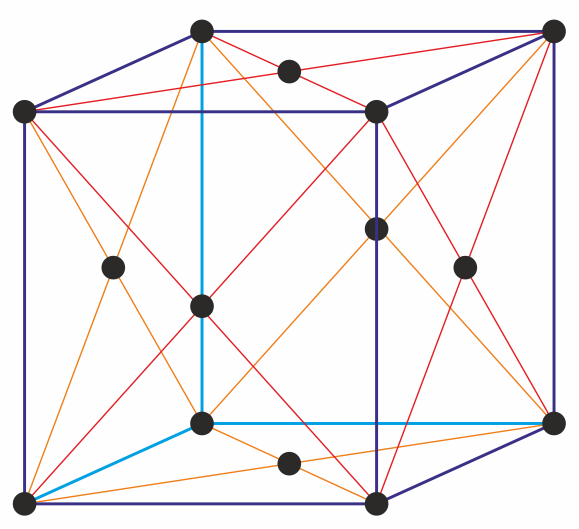
\includegraphics[width=0.5\textwidth]{figs/FCC.png}
    \caption{A schematic depiction of a face-centred cubic lattice portion. The gray dots are the desired locations of the Argon atoms in the solid state.}
    \label{fig: FCC}
\end{figure}

This is the most complex configuration of Argon. For the liquid phase, we expect a middle ground between the gas and solid phase configurations. 

Since the solid phase configuration is the most complex, we expect it to also be the most difficult to form. Hence, we will use the FCC-lattice as the initial positions of our Argon atoms. Should we wish to simulate solid phase Argon, the atoms are already in the right positions, and should we wish to simulate the other phases, the atoms more easily relocate to the newly desired configuration.

\raggedbottom
\newpage

\subsubsection{Velocity}

Initially, we allowed the initial velocities to be of some random magnitude and direction, with a homogeneous distribution. But using statistical physics we know that in the real world this not the case. As per the classical interpretation, velocities of particles are dependent on the temperature of the surrounding environment. More precisely, the magnitude of each velocity component $v_x$ follows a Maxwellian distribution, a Gaussian,

\begin{equation}
    p(v_x) \propto \exp\left(-\frac{m_\mathrm{Ar}v_x^2}{2k_\mathrm{B}T}\right)
    \label{eqn: Maxwell Distribution},
\end{equation}

where $p(v_x)$ is the probability of finding the magnitude $v_x$ of the $x$-component of the velocity. So we should expect our simulation to obey this distribution as well, and hence we draw random velocities according to the Maxwell distribution.

Unfortunately, there is one caveat. For Eqn. \ref{eqn: Maxwell Distribution} to hold in our simulated system we require a large number of Argon atoms, far too many for us to simulate in any reasonable amount of time. Consequently, since Eqn. \ref{eqn: Maxwell Distribution} holds for an environment in thermal equilibrium, our simulated system will most likely not be in thermal equilibrium. For it then to transform to being in equilibrium, the Argon atoms will need to interact and exchange energy, a process which, again, can take an enormous amount of time. We accelerate this process by the nudging the velocities of each Argon atom in the right direction.

One other result from statistical physics is that the total kinetic energy of a system is approximately given by,

\begin{equation}
    E_\mathrm{kin} = (N-1)\frac{3}{2}k_\mathrm{B}T,
    \label{eqn: Target Kin-E}
\end{equation}

with $N$ the number of particles in the system. Like before, this equation only holds for a system containing a large number of particles. However, we can use this theoretical kinetic energy as a target energy for our simulated system, such that it more closely follows reality. Should we find that our simulated system has a total kinetic energy close to the target energy, we can safely assume that our simulated system is (close to being) in equilibrium. On the contrary, should we find that the simulated total kinetic energy deviates substantially from the target kinetic energy, we change the velocities of the Argon atoms according to the scaling parameter $\lambda$,

\begin{equation}
    \lambda = \sqrt{\frac{(N-1)3k_\mathrm{B}T}{\sum_i m_\mathrm{Ar}v_i^2}},
    \label{eqn: lambda}
\end{equation}

with the $\sum_i m_\mathrm{Ar}v_i^2$ term corresponding to the total kinetic energy of our simulated system. Using $\lambda$, we scale all velocities of our Argon atoms equally $(\vec{v}_i \rightarrow \lambda \vec{v}_i)$. 

\raggedbottom
\newpage

The important part of this process is to do it after the simulation has already run for several integration steps, doing this allows the Argon atoms to already exchange some energy with each other. 

This process of finding the correct initial velocities we called "equilibration", and can be summarized in 5 steps:
\begin{enumerate}
    \item Draw a velocity for each Argon atom, following the Maxwellian distribution given in Eqn. \ref{eqn: Maxwell Distribution}.
    \item Run the simulation for several integration steps, we chose to run it for 10 integration steps during the equilibration process.
    \item Determine the total simulated kinetic energy.
    \item If the total simulated kinetic energy deviates significantly from the target kinetic energy (see Eqn. \ref{eqn: Target Kin-E}), rescale the velocities of all Argon atoms by $\lambda$ (see Eqn. \ref{eqn: lambda}). We used a tolerance of 5\% to determine whether the simulated kinetic energy deviates significantly from the target kinetic energy.
    \item Repeat steps 2-4 until the simulated total kinetic energy is within the desired tolerance of the target kinetic energy.
\end{enumerate}

Using the initial FCC-positions and performing the equilibration process will result in a system of Argon atoms in equilibrium with the surrounding thermal bath, and now better represents Argon in the corresponding state of matter. From here onwards, the true simulation can begin.

\subsection{Observables}

We have already discussed that we are able to extract energies from our simulation, and thus can observe intrinsic properties of our simulated system. In this section, we describe two more properties we can observe from our simulated system: pair correlation and pressure.

\subsubsection{Pair Correlation}
\label{sec: Pair Correlation}

Depending on the initial conditions, in order to minimize their energy, Argon atoms will arrange themselves into different configurations. These are the three familiar states of matter: solid, liquid and gas. In order to quantify the difference between these  states we calculate the distribution of distances between pairs of Argon atoms. This is done via the pair correlation distribution $g(r)$,

\begin{equation}
    g(r) = \frac{2L^3}{N(N-1)}\frac{\left\langle n(r)\right\rangle}{4\pi r^2 \Delta r},
    \label{eqn: Pair Correlation}
\end{equation}

\raggedbottom
\newpage

where $L$ is the box size, $N$ the number of Argon atoms, $\Delta r$ by how much we increase the distance $r$ each step (the bin size), and $n(r)$ counts how many Argon atoms we encounter in the interval $\left[r, r+\Delta r \right]$. $\langle \;\rangle$ indicates an average over configurations. Where a configuration can either be a snapshot of the simulation at a different integration step, or a different simulation with the same initial density and temperature but different initial positions and velocities.

In our collection of Argon atoms, we pick a reference atom and from there we move radially outwards and count how many other atoms we encounter over distance. Doing this for all Argon atoms and summing the results gives the $n(r)$ for one integration step. Doing this for many integration steps during the simulation and then averaging the results gives $g(r)$. For this process, we expect a different result for each state of matter. 

As we have established before, for the solid state of matter, from lab observations it is known that Argon atoms form a regular crystal structure following the FCC configuration. Due to this regular structure, we only expect to encounter other Argon atoms at very regular distances, hence $g(r)$ for solid state Argon would look like a collection of Dirac-delta functions ("Barcode"). 

We know the gas to be the most energetic state of matter, hence the average energy per Argon atom in our simulations should be very high for a gas. This high energy causes the Argon atoms to interact numerous times during the simulation, eventually settling down into a structure which distributes the atoms as homogeneously as possible. Hence, we expect $g(r)$ for a gas state simulation of Argon to be relatively flat over distance, since the likelihood of finding an Argon atom at any distance should be constant. In fact, the prefactors in Eqn. \ref{eqn: Pair Correlation} have been tuned in such a manner that for a gas we expect $g(r) \approx 1$.

For the liquid state, we expect $g(r)$ to follow similar behaviour as Argon on a macro level, namely, that it inherits properties of both the solid and gas state. This gives that $g(r)$ is relatively constant; no sharp peaks, like a gas. But does rise and fall gradually over distance, like a solid.  

\subsubsection{Pressure}

From a classical point of view, pressure would be the average force exerted on the boundary of our simulation box. However, since we are considering our box to be infinite by the minimal image convention, we need to use a different way of calculating the pressure of our simulated system, namely, an adapted version of the equation for pressure $P$ given in Verlet 1967 \cite{verlet1967computer},

\begin{equation}
    \frac{P}{k_\mathrm{B}Tn} = 1 - \frac{1}{6Nk_\mathrm{B}T} \left\langle \sum_i \sum_{j>i} r_{ij}\frac{\partial V_\mathrm{LJ}(r_{ij})}{\partial r}\right\rangle,
    \label{eqn: Pressure}
\end{equation}

\raggedbottom
\newpage

where $n$ is the number density of Argon atoms, and $\langle \;\rangle$ is again the average over configurations. Eqn. \ref{eqn: Pressure} consists of two parts: the 1 encodes the ideal gas law, as per the factors on the left-hand-side, and the sum-part encodes the change in pressure due to interactions occurring between Argon atoms, as per the Lennard -- Jones potential $V_\mathrm{LJ}$. Using Eqn. \ref{eqn: Pressure}, we determined pressures for our simulations by calculating $\sum_i \sum_{j>i} r_{ij}\frac{\partial V_\mathrm{LJ}(r_{ij})}{\partial r}$ at each integration step corresponding to 10\% of the total number of integration steps, and afterwards averaging each calculated sum-part to get the total pressure of our simulated system.

\subsection{Triple Point}
Whether or not matter exists in a certain phase depends on its pressure and temperature. However, the boundaries between two phases are not clear cut. Take water as an example. Its freezing point is at 0$\degree$C, but if we placed some of it in 0.5 $\degree$C -and atmospheric pressure- some of it would be a solid and some of it would be liquid. The two phases are allowed to co-exist. \\ \\
Pushing this idea, we can imagine that there should be a point in the Temperature-Pressure parameter space where all three phases co-exist. In order to find this sweet-spot in the parameter space, we use our simulation code as an experimental bench. We calculated the pressure and deduced which phase of matter argon is in through the pair correlation function for multiple initial condition. We did not conduct an exhaustive search, but rather took advantage of the known shape ($\Upsilon$) of the transition lines. Thus, we attempted to find where the transition lines are and follow them to the triple point.
\section{Results}
\label{sct: Results}
We ran 3 simulations, each corresponding to a different phase of matter for our Argon atoms. The initial conditions of these simulations are summarised in Tab. \ref{tab: Initial Conditions}. 

{\renewcommand{\arraystretch}{1.2}
\begin{table}[H]
    \centering
    \begin{tabular}{c||c|c|c|c}
    \multirow{2}{*}{State} & \multicolumn{2}{c|}{Temperature} & \multicolumn{2}{c}{Density} \\
    \cline{2-5}
         & $[k_\mathrm{B}\varepsilon]$ & $[\mathrm{K}]$ & $\left[m_\mathrm{Ar}\;\sigma^{-3} \right]$ & $\left[\si{g.cm^{-3}}\right]$ \\
    \hline
       Solid  & 0.5 & 59.90 & 1.20 & 2.01\\
       Liquid & 1.0 & 119.8 & 0.80 & 1.34\\
       Gas    & 3.0 & 359.4 & 0.30 & 0.50\\
    \end{tabular}
    \caption{Initial conditions. Each simulation was also run using 108 Argon atoms, ran over $10\ssi{ps}$, and with a time step of $0.001\ssi{ps}$.}
    \label{tab: Initial Conditions}
\end{table}
}

\raggedbottom
\newpage

These initial conditions were confirmed to correspond to their associated state, as per Tab. \ref{tab: Initial Conditions}. For each simulation, an energy-evolution figure was created as a check to see if the simulation behaved as expected. The energy-evolution figure for the Gas-state simulation is given in Fig. \ref{fig: Energy Evolution}.

\begin{figure}[H]
    \centering
    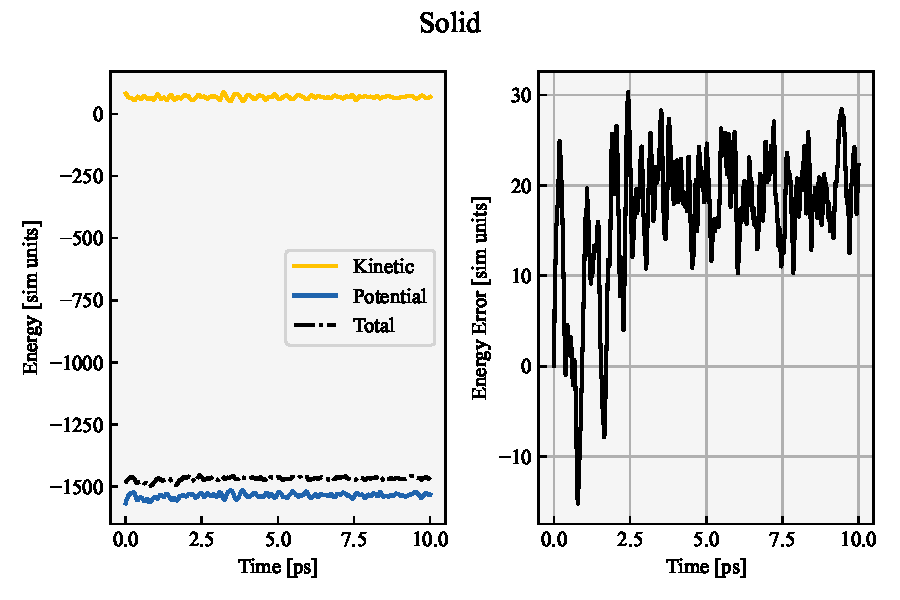
\includegraphics[width=1\textwidth]{figs/energy_err.pdf}
    \caption{Total energies of the Argon atoms during the simulation for the Gas simulation given in Tab. \ref{tab: Initial Conditions}. }
    \label{fig: Energy Evolution} 
\end{figure}

The most important thing to note in Fig. \ref{fig: Energy Evolution} is that the total energy, the black dash-dotted line in the left panel, is relatively constant over the course of the simulation. This indicates that we have done the integration correctly, since the Verlet algorithm 
approximately conserves energy. All simulations with the initial conditions given in Tab. \ref{tab: Initial Conditions} produced similar energy-evolution figures.

For each simulation, we created an additional figure, the pair correlation distribution over distance, as can be seen in Fig. \ref{fig: Pair Correlation}.

\raggedbottom
\newpage

\begin{figure}[H]
\centering

\begin{subfigure}{0.49\textwidth}
    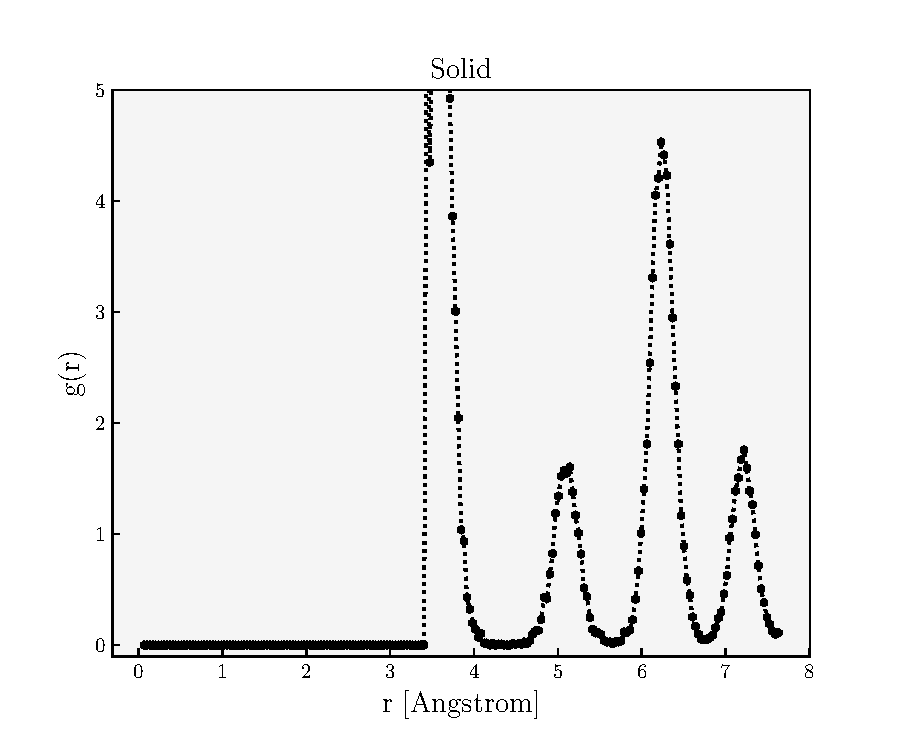
\includegraphics[width = 1\textwidth]{figs/solid.pdf}
    \caption{Solid}
    \label{fig: Solid}
\end{subfigure}
\begin{subfigure}{0.49\textwidth}
    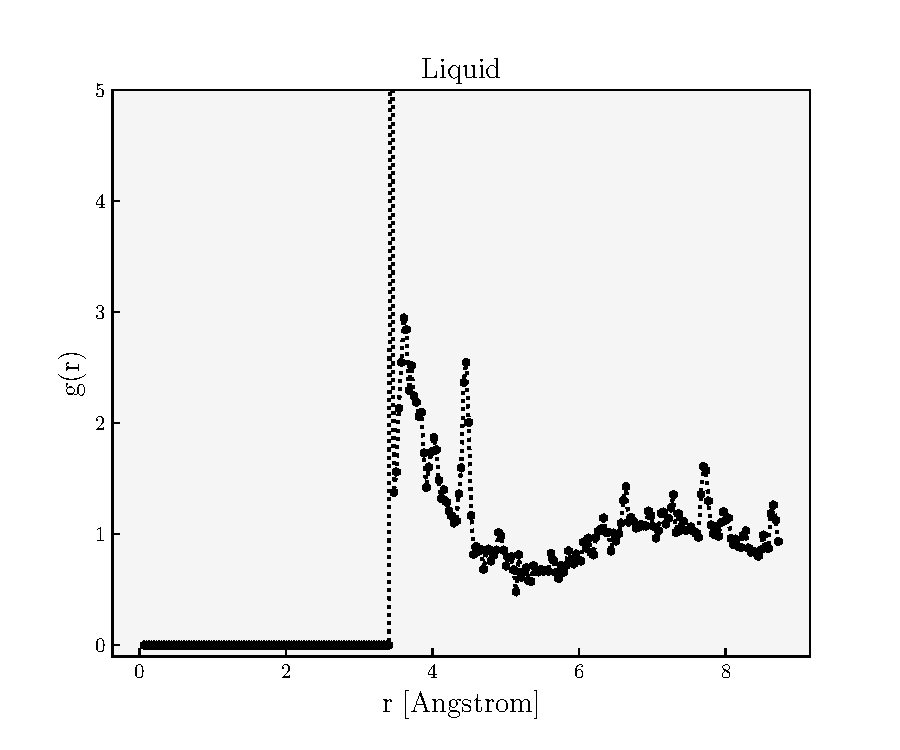
\includegraphics[width = 1\textwidth]{figs/liquid.pdf}
    \caption{Liquid}
    \label{fig: Liquid}
\end{subfigure}
\begin{subfigure}{0.49\textwidth}  
    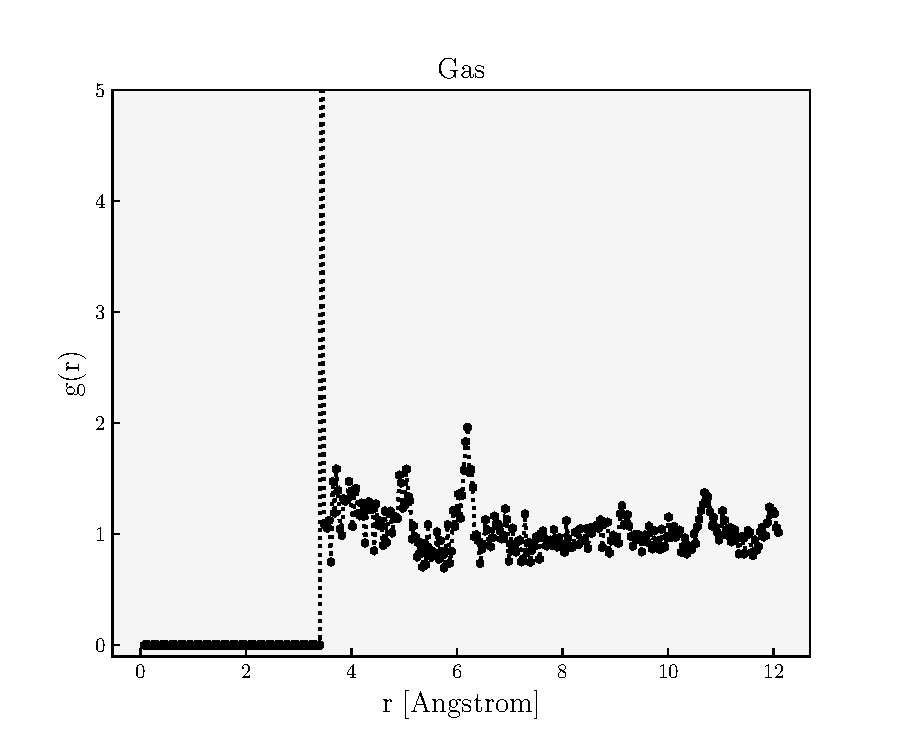
\includegraphics[width = 1\textwidth]{figs/gas.pdf}
    \caption{Gas}
    \label{fig: Gas}
\end{subfigure}
\caption{Pair Correlation distribution over distance for each simulated state.}
\label{fig: Pair Correlation}
\end{figure}

The main things to note are the distinctive shapes of the pair correlation distributions of the solid and gas states (Figs. \ref{fig: Solid} and \ref{fig: Gas} respectively). As we have established in Sec. \ref{sec: Pair Correlation}, for the solid state simulation we expect other Argon atoms to only appear at certain distances with respect to the reference Argon atom, giving rise to the barcode-like shape given in Fig. \ref{fig: Solid}. 

As established in Sec. \ref{sec: Pair Correlation}, in the gas phase, the Argon atoms are the most unbound from one another and thus distribute themselves nearly homogeneously, giving rise to a relatively constant probability of finding an Argon atom a certain distance from another Argon atom, hence the flat pair correlation distribution given in Fig. \ref{fig: Gas}. 

As expected, the liquid pair correlation distribution (see Fig. \ref{fig: Liquid}) shares aspects of both the solid and gas state pair correlation distribution.

In summary: Our generated pair correlation distributions match our intuition, indicating that the initial conditions given in Tab. \ref{tab: Initial Conditions} correspond to their respective states.

\raggedbottom
\newpage

Lastly, we calculated the average pressure of each of our simulated systems, as per Eqn. \ref{eqn: Pressure}, the mean values and standard deviations of which are given in Tab. \ref{tab: Pressures Results}. 

{\renewcommand{\arraystretch}{1.2}
\begin{table}[H]
    \centering
    \begin{tabular}{c||c|c}
         \multirow{2}{*}{State} & \multicolumn{2}{c}{Pressure} \\
         \cline{2-3}
         & $\left[k_\mathrm{B}\varepsilon\;\sigma^{-3} \right]$ & $\left[\times10^{9}\ssi{erg.cm^{-3}} \right]$\\
         \hline
         Solid & $8.0 \pm 0.3$ & $3.3 \pm 0.1$\\ % 7.919 +/- 0.330, 3.317 +/- 0.138
         Liquid & $1.0 \pm 0.3$ & $0.4 \pm 0.1$ \\
         Gas & $0.9 \pm 0.1$ & $0.38 \pm 0.04$\\
    \end{tabular}
    \caption{Measured pressures and standard deviations for the 3 simulated collections of Argon atoms for different states, as per Tab. \ref{tab: Initial Conditions}.}
    \label{tab: Pressures Results}
\end{table}
}
Next, we present the phase space of Argon, as we calculated it from our numerical experiments.

\begin{figure}[H]
    \centering
    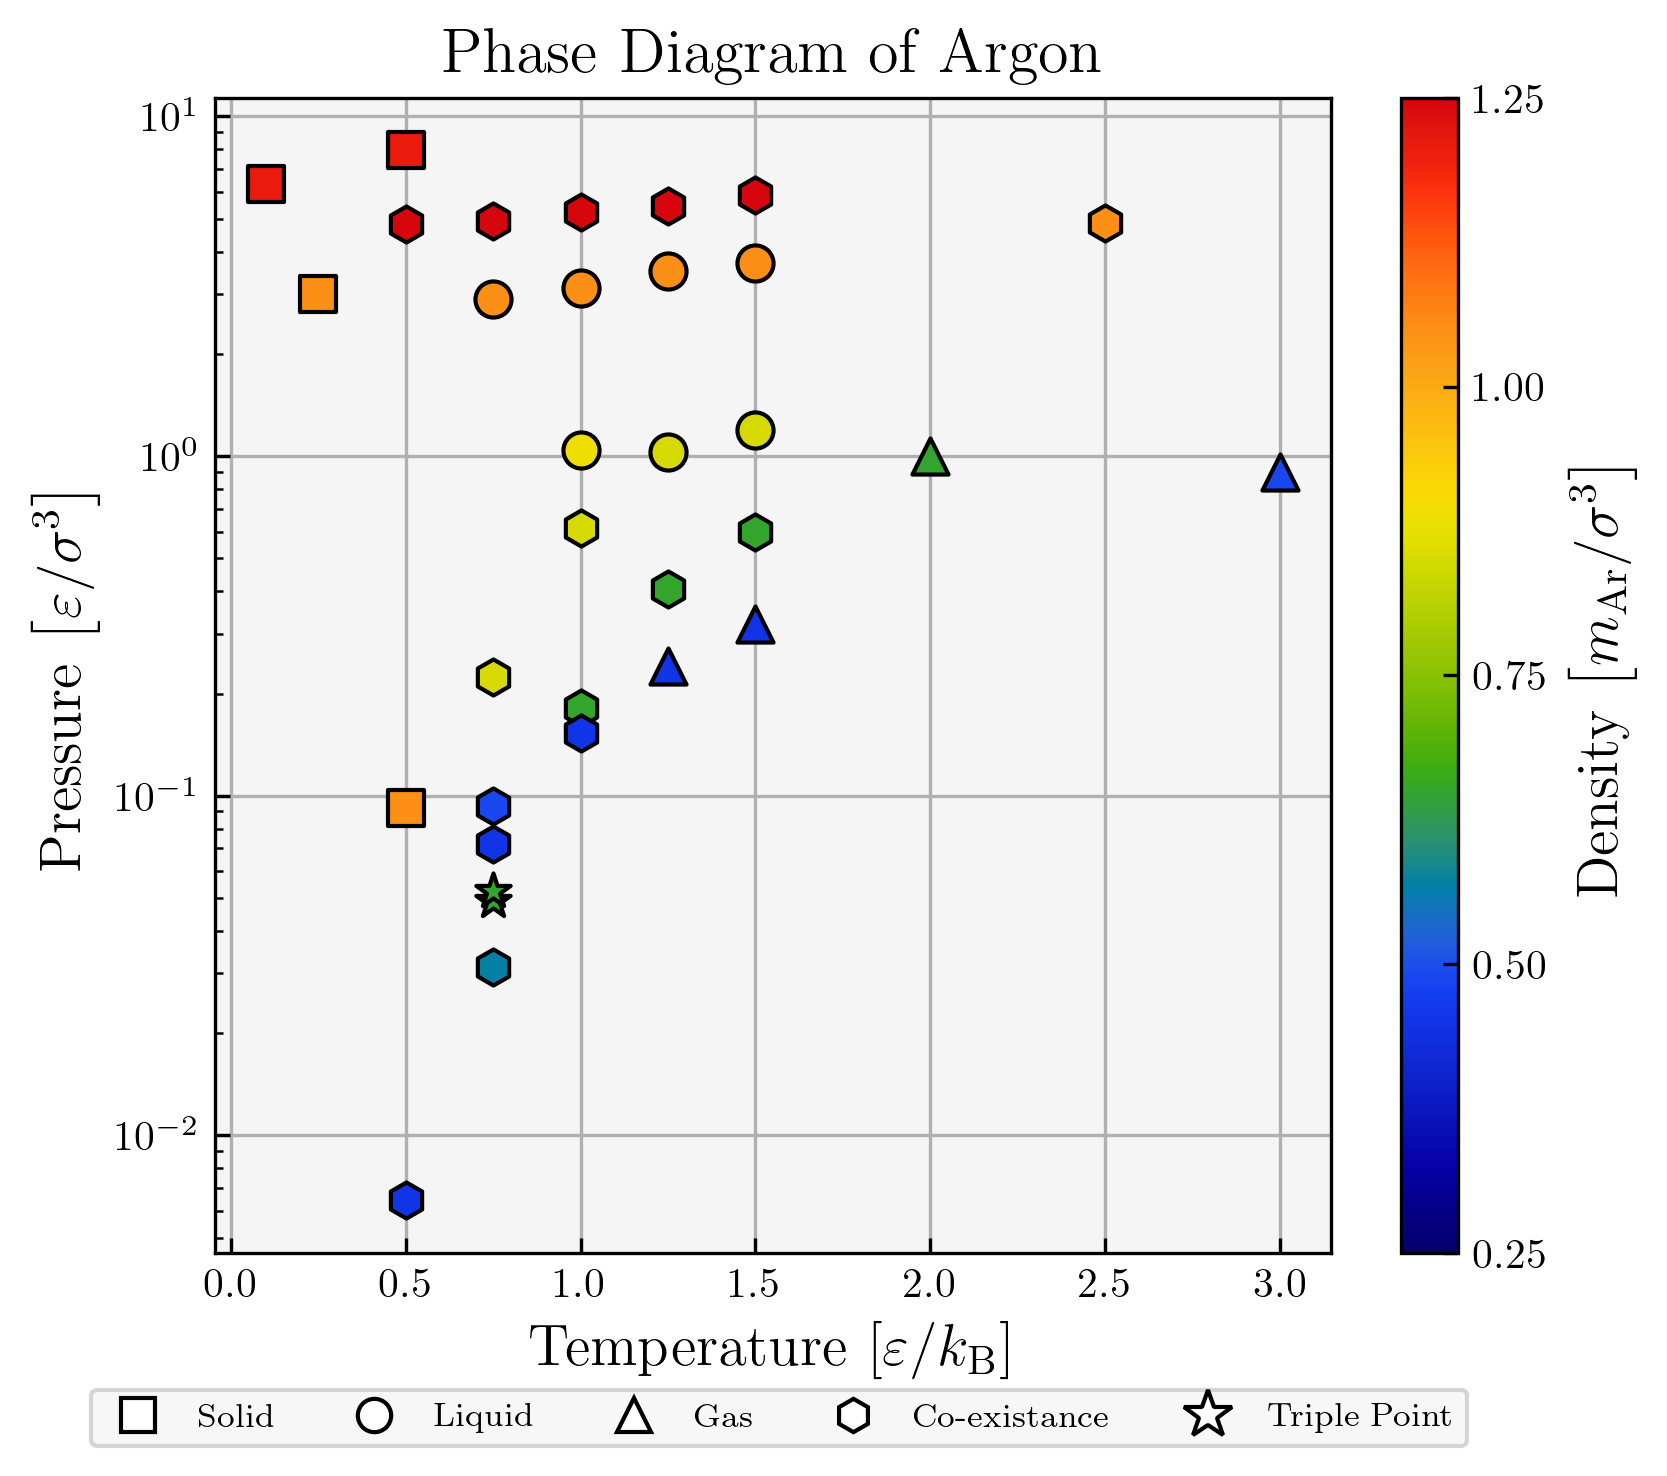
\includegraphics[width=0.75\textwidth]{figs/our_phase_space.png}
    \caption{Phase space of Argon. X-axis is the temperature, y-axis is the pressure, color scale corresponds to density. Different markers signify different phases of matter, or coexistance. When three phases co-existed, we deduced it is the triple point.}
    \label{fig: phasespace}
\end{figure}

Our deduced triple point (T,P) = (0.75 $k_\mathrm{B}\varepsilon$, 0.004 $k_\mathrm{B}\varepsilon \sigma^{-3}$) = (90 K , 10$^{\text{-4}}$ $\pm$ 9$\times $10$^{\text{-4}}$ GPa) agrees with the literature value \cite{triplepoint} of a Lennard -- Jones Argon atom (T,P) = (0.69 $k_\mathrm{B}\varepsilon$, 0.001 $k_\mathrm{B}\varepsilon \sigma^{-3}$) and with the experimentally deduced value, as is evident in Fig. \ref{fig: phasespace}.

\raggedbottom
\newpage

\begin{figure}[H]
    \centering
    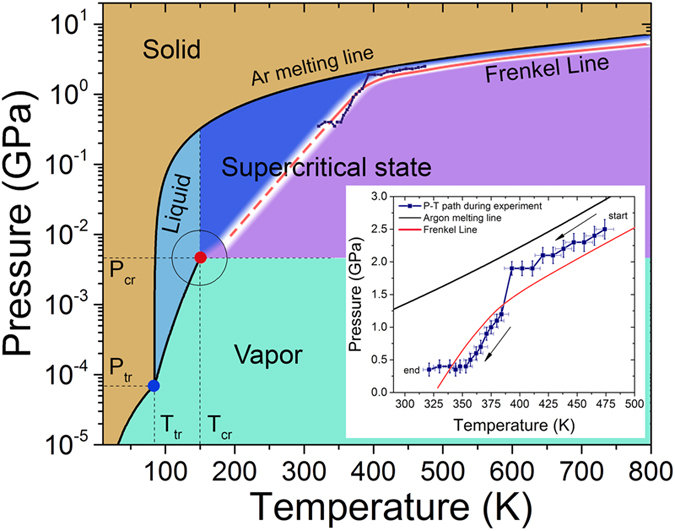
\includegraphics[width=0.75\textwidth]{figs/phase_space.jpeg}
    \caption{Experimentally determined phase space of Argon, adapted from Bolmatov et al. (2015) \cite{phasespace}.}
    \label{fig:phasespace}
\end{figure}

\begin{figure}[H]
    \centering
    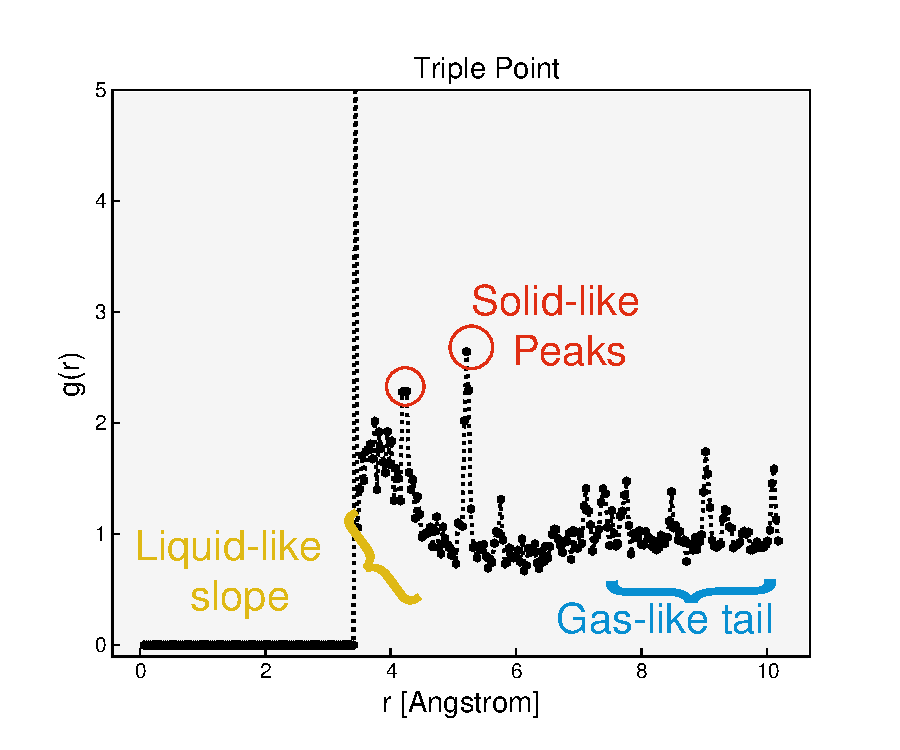
\includegraphics[width=0.75\textwidth]{figs/triple_point.pdf}
    \caption{The pair correlation function for our triple point, (T,$\rho$) = (0.75 $k_\mathrm{B}\varepsilon$, 0.5 $m_\text{Ar} \sigma^{-3}$). It exhibits characteristics found in all three phases of matter.}
    \label{fig:enter-label}
\end{figure}

\raggedbottom
\newpage

\section{Summary}
\label{sct: Discussions}

We present here a tentative summary of how we executed Project 1: Molecular Dynamics of the MSc course Computational Physics given in the year 2024 at Leiden University.

\begin{enumerate}
    \item We built a code collection capable of simulating Argon atoms contained inside a pseudo-infinite box, as by the minimal image convention. 
    
    \item Our basis for the simulation lies in the usage of the Lennard -- Jones potential (see Eqn. \ref{eq:LJ}) and implementing the Verlet integration algorithm (see Eqns. \ref{eqn: Verlet Vel} and \ref{eqn: Verlet Pos}).
    
    \item As to more accurately describe the macro observations of Argon in different states, we implemented the face-centred cubic lattice as the initial positions of our Argon atoms in the simulation.

    \item For similar reasons, we implemented a setup-stage before the simulation (equilibration), so that the velocities of the Argon atoms more closely follow what we would expect to see for a large number of atoms. 

    \item Having run the simulations for each state of matter (see Tab. \ref{tab: Initial Conditions}), we created two figures for each state: the energy-evolution and pair correlation distribution. Each figure matched what we intuitively would expect.

    \item For each ran simulation, we calculated the mean pressure and its standard deviation via Eqn. \ref{eqn: Pressure}, the results of which are showcased in Tab. \ref{tab: Pressures Results}. 

    \item By running large grids of simulations, we were able to create a phase diagram of Argon and were able to deduce that the triple point of Argon occurs at (T,P) = (90 K , 10$^{\text{-4}}$  $\pm$  9$\times $10$^{\text{-4}}$ GPa).
\end{enumerate}

\bibliographystyle{siam}
%\nocite{*} % show all citations, regardless if they're used in the report.

\section*{Bibliography}
{
\renewcommand{\clearpage}{} 
\begingroup
\renewcommand{\section}[2]{}%
\bibliography{References}
\endgroup
}

\end{document}
